%-------------------------------
%-------------------------------
\chapter{Zusätzliche Funktionen}
\label{chapter:additional_features}

In Kapitel \ref{chapter:skeleton_generation} wird beschrieben wie der Algorithmus abläuft. In diesem Kapitel geht es nun darum die Verwendungsmöglichkeiten des Algorithmus auszuschöpfen. Über eine Benutzeroberfläche wird die Bedienung vereinfacht und gezeigt welche Möglichkeiten es gibt die Skelettgenerierung zu steuern. Außerdem ist es möglich die Metadaten eines Skeletts zu speichern und Variationen zu einem bestehenden Skelett zu generieren.


%---------------------------
\section{Benutzeroberfläche}
\label{gui}

Mit dem in Kapitel \ref{chapter:skeleton_generation} vorgestellten Algorithmus können nicht nur zufällige Skelette generiert werden. Über eine Benutzeroberfläche ist es auch möglich, dem Algorithmus zusätzliche Eingaben zu geben. Die Benutzeroberfläche ist in Abbildung \ref{gui_screenshot} zu sehen.

\begin{figure}
 \centering
 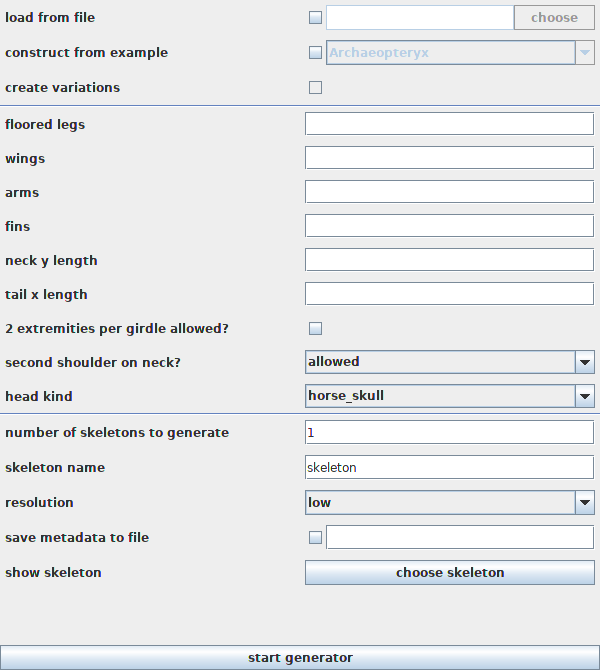
\includegraphics[width=0.7\textwidth]{graphics/gui.png}
 \caption{Die Benutzeroberfläche des Programms. Der Knopf "`start generator"' startet den Algorithmus mit den zusätzlichen Eingaben aus den Feldern darüber.}
 \label{gui_screenshot}
\end{figure}

Diese Eingaben werden unter anderem in Bedingungen umgewandelt, die schon von der PCA berücksichtigt werden. Wie eine bedingte Verteilung als Eingabe für die PCA berechnet wird, wird in Abschnitt \ref{pca_conditions} erklärt. Wie dort auch beschrieben, werden bei allen Bedingungen zufällige kleine Werte aufaddiert oder abgezogen um mehr Variation auf den erzeugten Skeletten zu bekommen. Dies ist sinnvoll, da der Benutzer so nicht gezwungen wird so etwas wie $1{,}4$ Beinpaare zu verlangen, um \zb die Form der Wirbelsäule zu verändern. Bei solch einer Eingabe müsste dann außerdem durch den Algorithmus ausgelost werden, ob das Skelett am Ende $1$ oder $2$ Beinpaare hat. Das wäre unter Umständen verwirrend.\\
Ist in Zahlenfeldern nichts eingegeben, haben diese keinen Einfluss auf den Ablauf (im Gegensatz zur Eingabe der Zahl $0$).

\begin{figure}
 \subfloat[$8$ Beine]{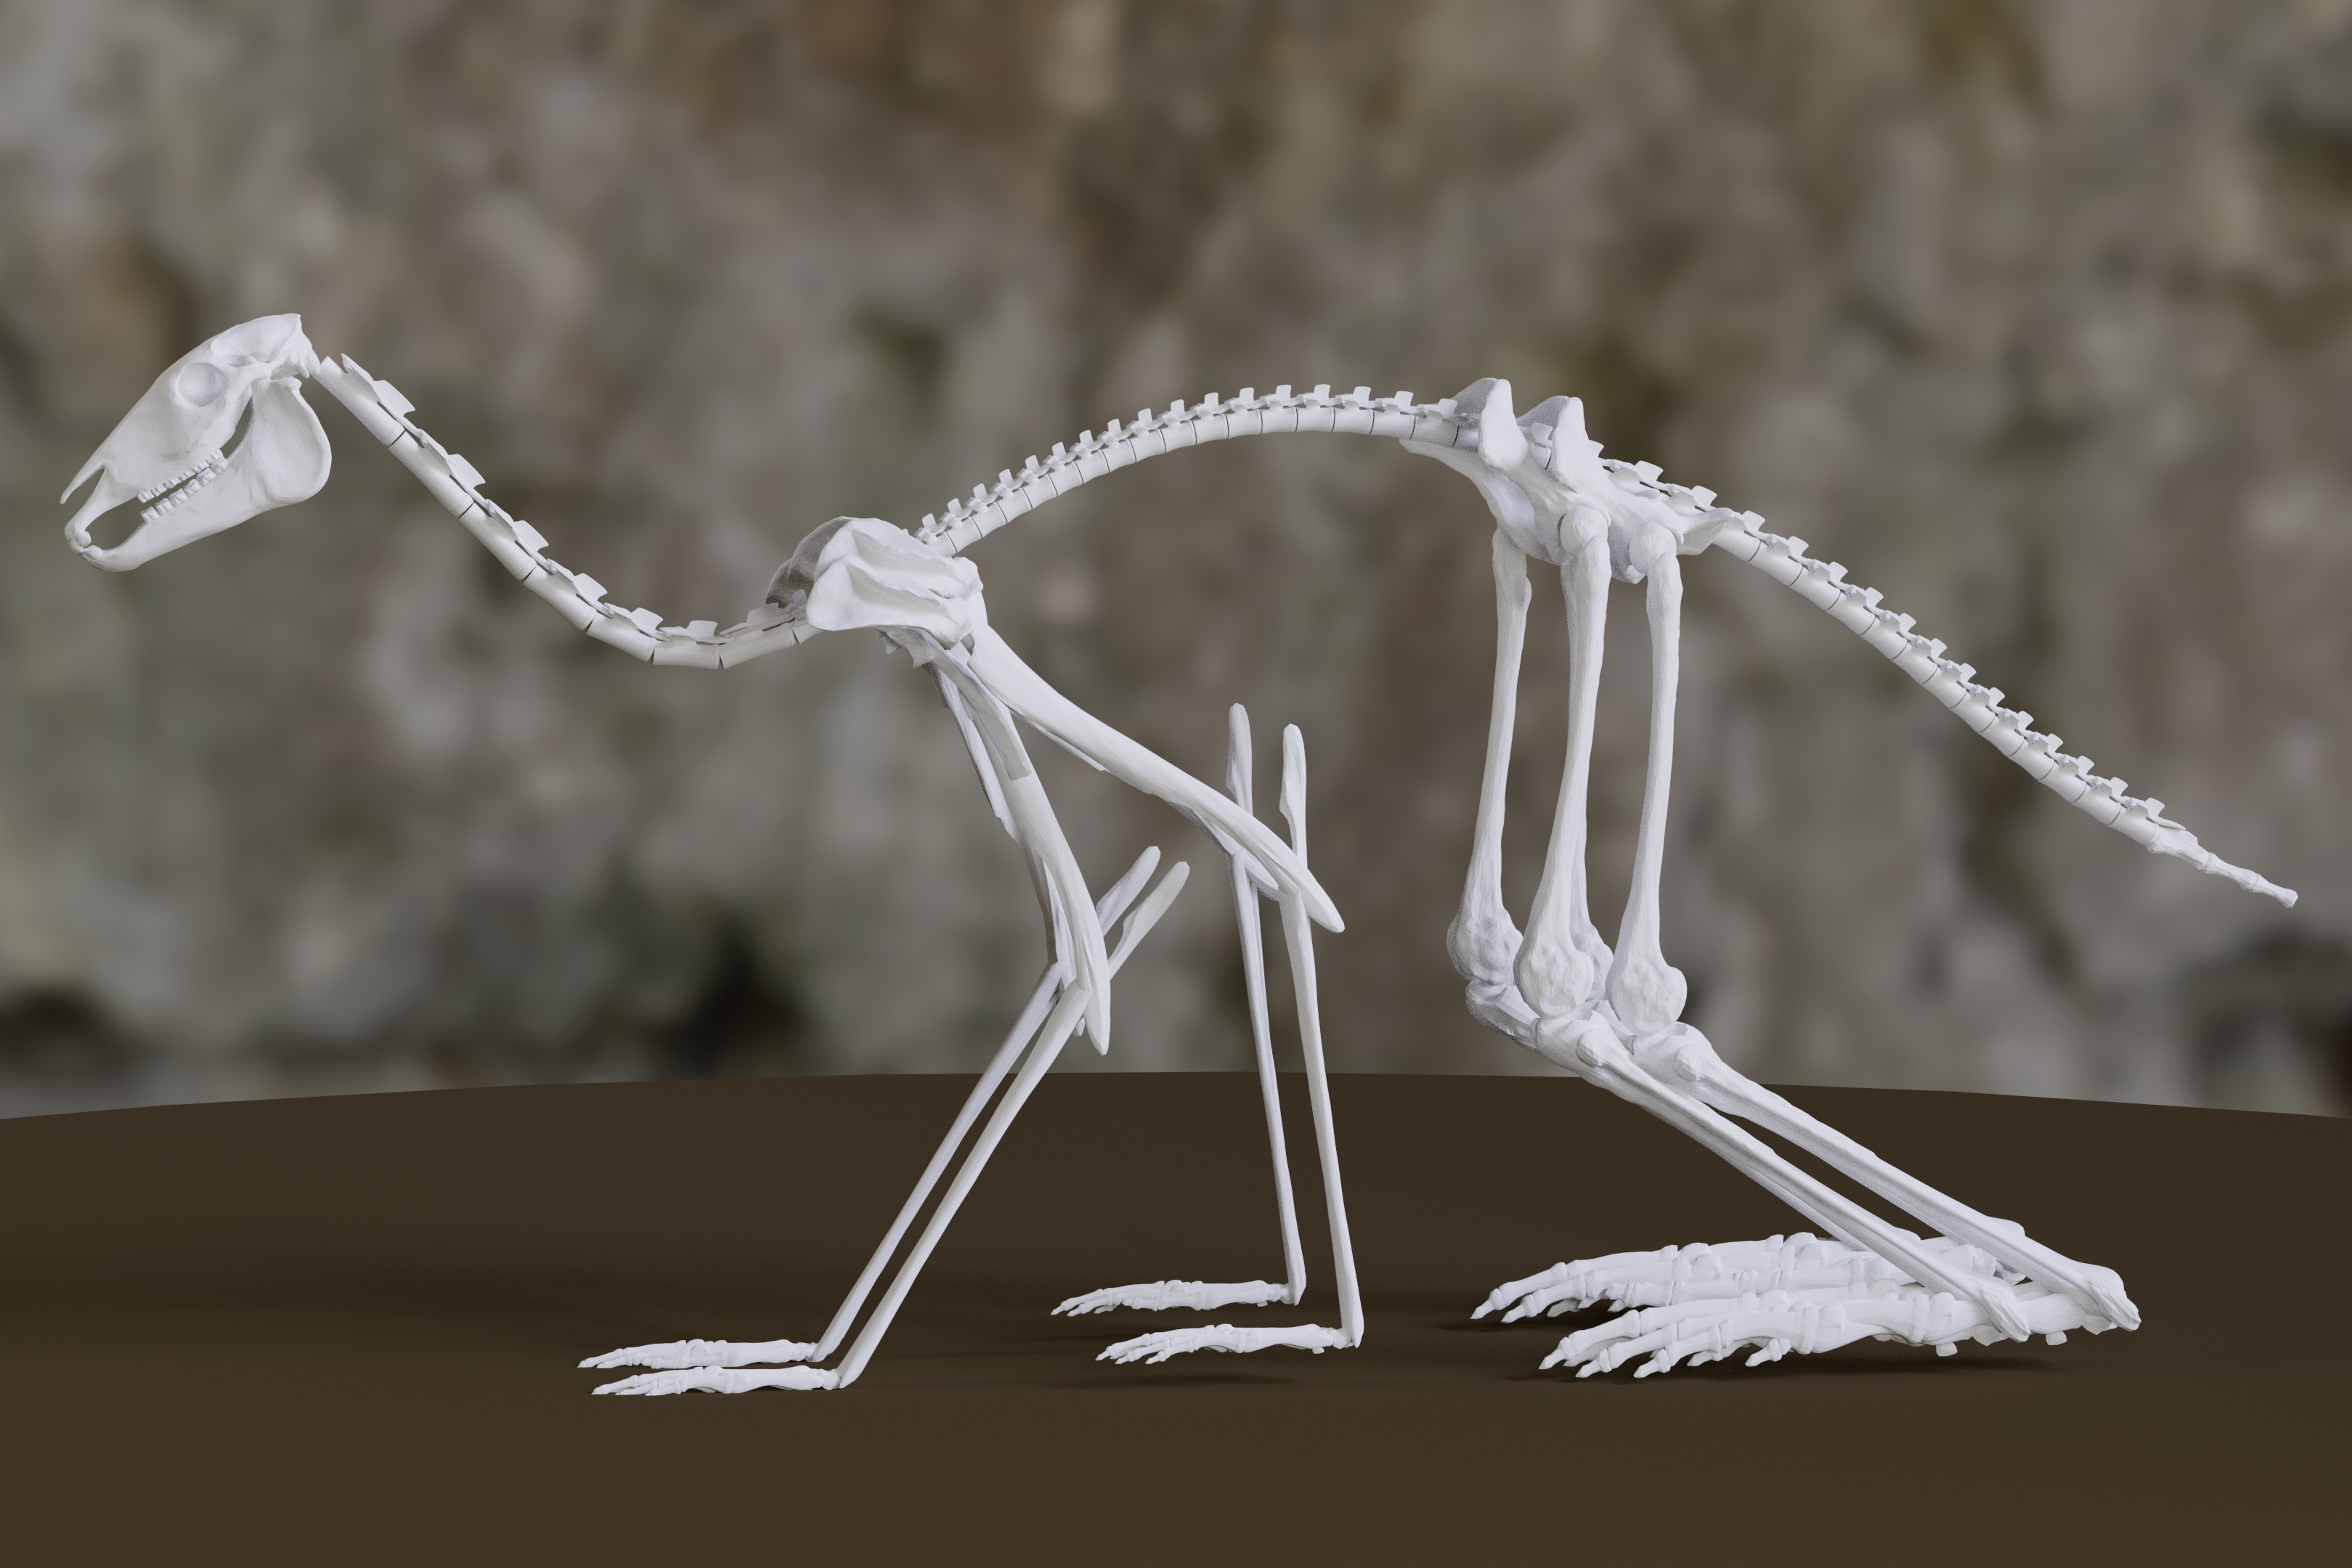
\includegraphics[height=5.8cm]{../java_skeleton_generation/example_skeletons/8legs.jpg}}~
 \subfloat[$1{,}5$ Flügel]{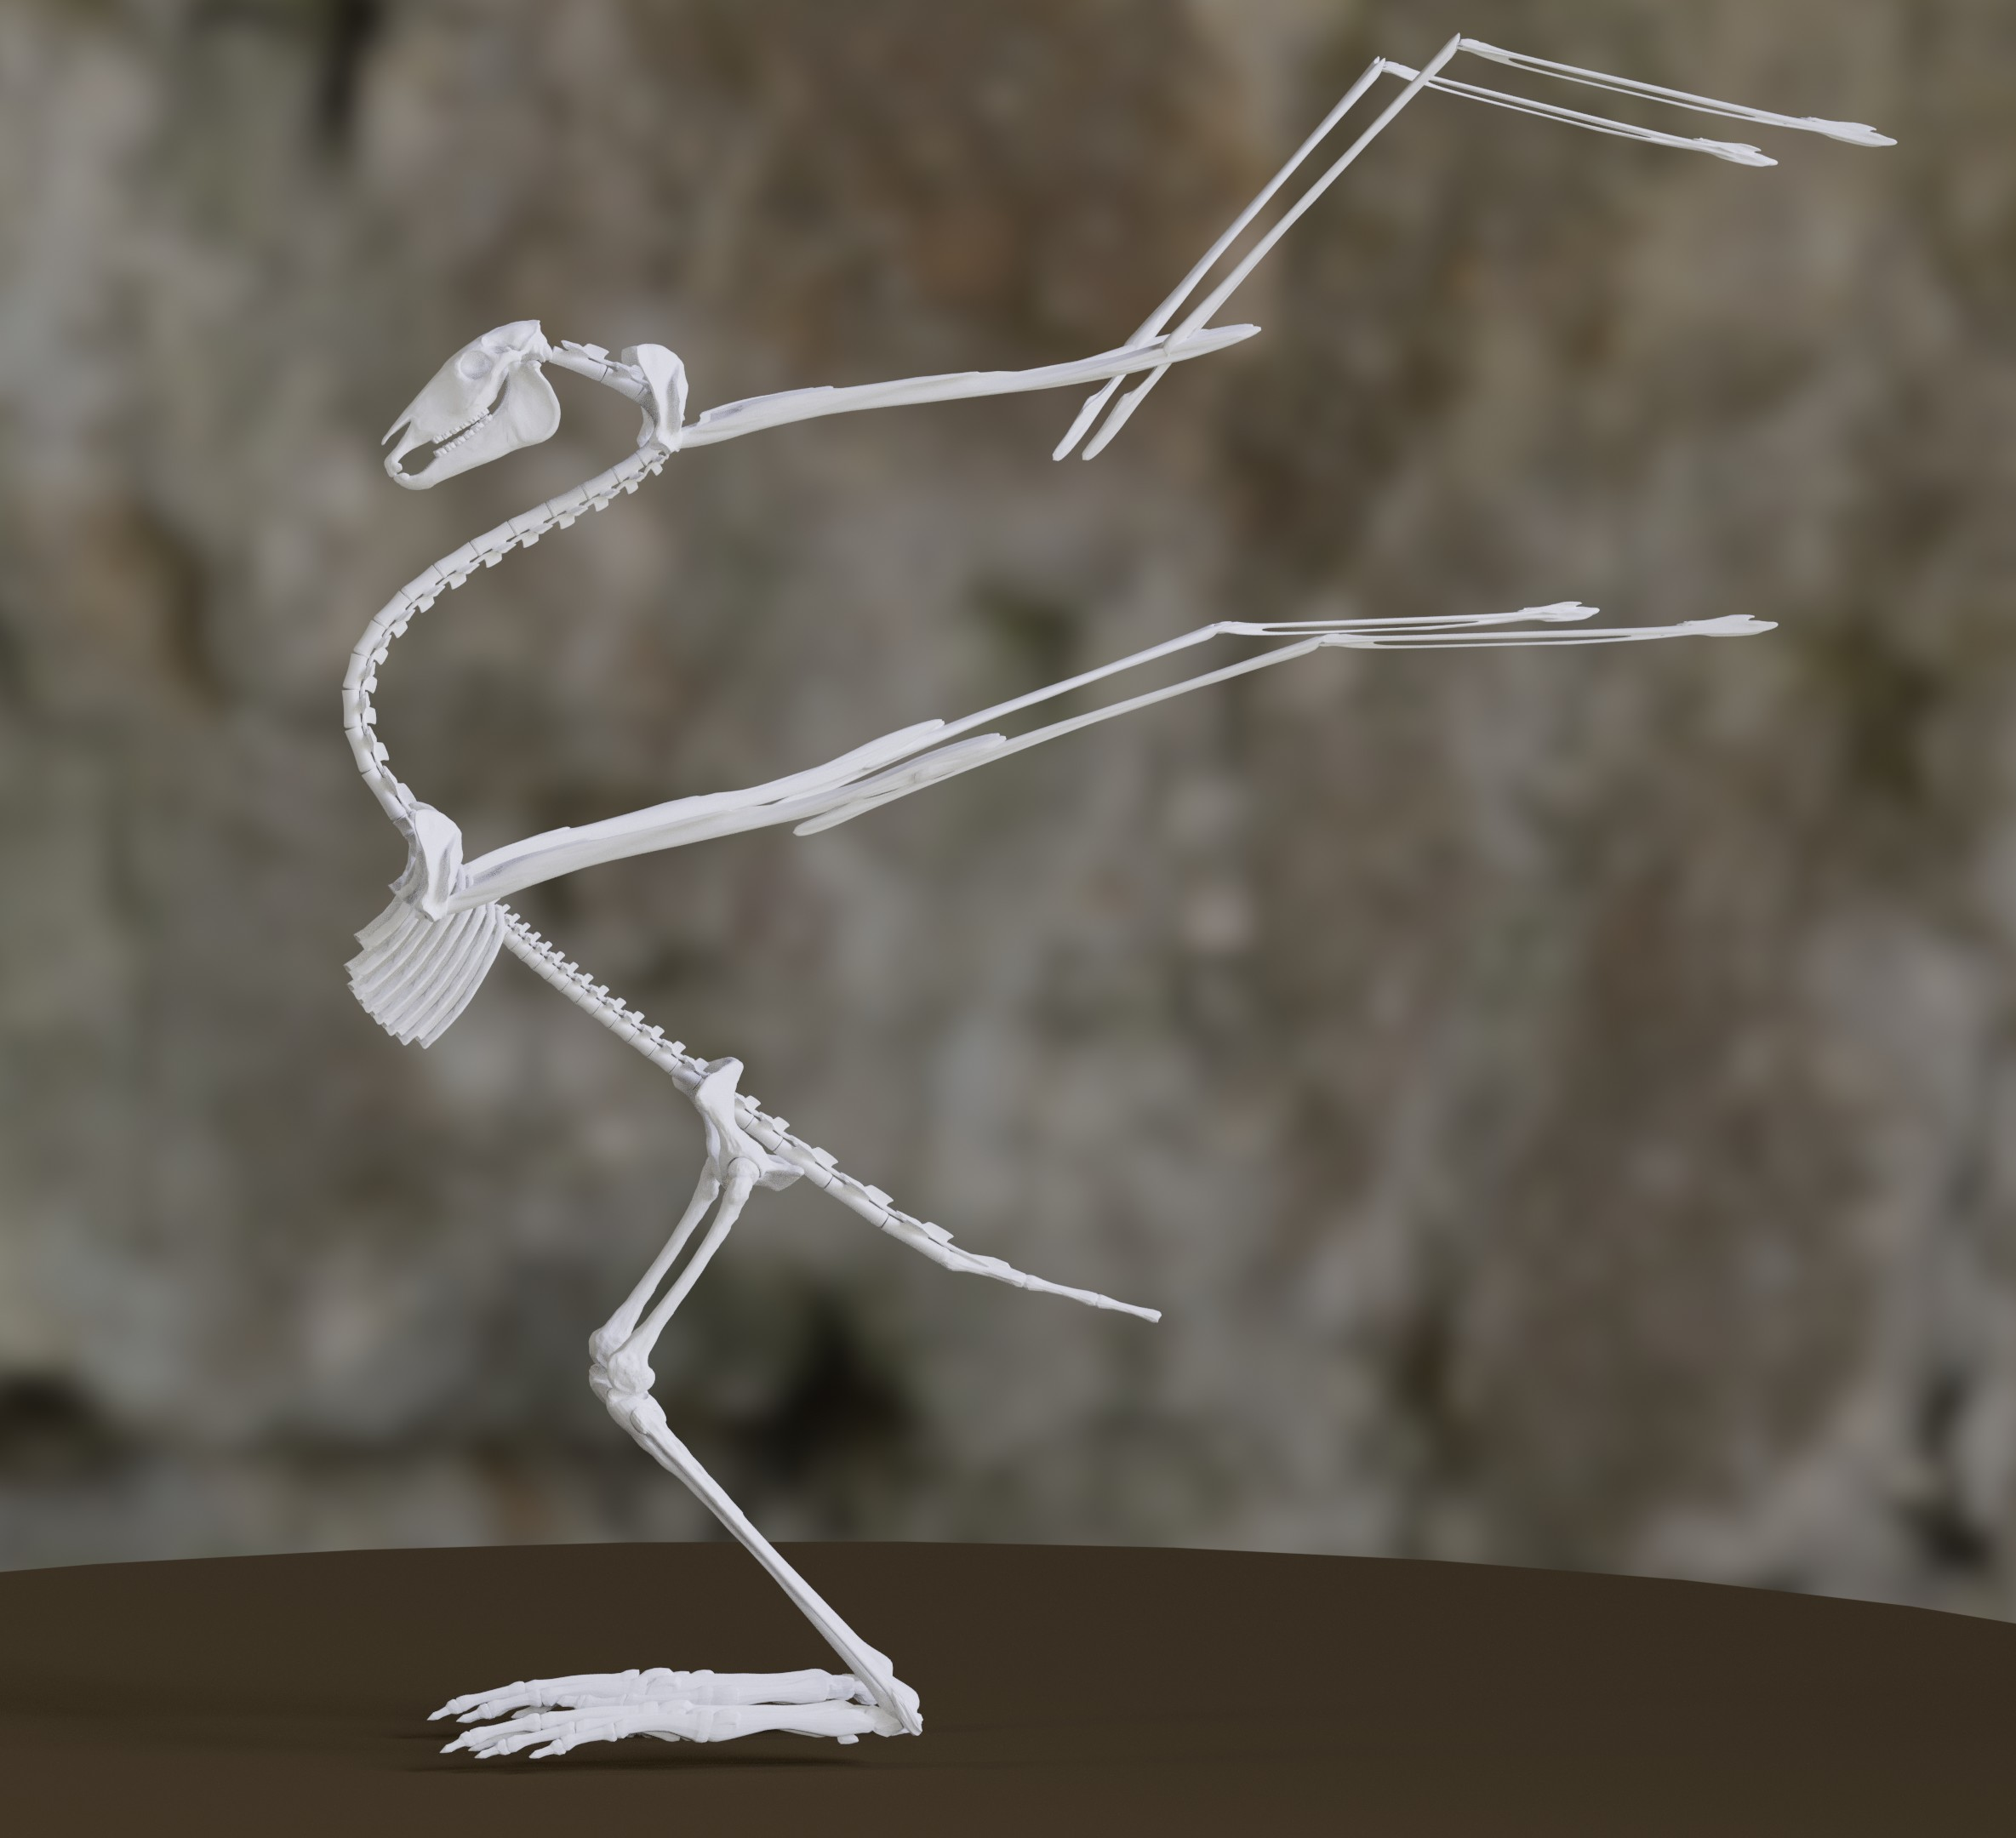
\includegraphics[height=5.8cm]{../java_skeleton_generation/example_skeletons/15wings.jpg}}
 
 \caption{Zwei Skelette, die mit extremen Bedingungen für die PCA generiert wurden. Als Hintergrund wurde \cite{background} verwendet. (a) Benutzereingabe: $8$ Beine und $4$ Beinpaare als Bedingung für \emph{Beine mit Bodenkontakt}. Es ist kein zweiter Schultergürtel am Hals erlaubt, aber zwei Extremitätenpaare pro Extremitätengürtel. (b) Benutzereingabe: $4$ Flügel und $1{,}5$ Flügelpaare als Bedingung für die PCA. Ein zweiter Schultergürtel am Hals wird erzwungen, aber es ist nur ein Extremitätenpaar pro Extremitätengürtel erlaubt.}
 \label{more_extremities}
\end{figure}

Die folgenden Eingaben werden durch die PCA berücksichtigt:
\begin{itemize}
 \item Die Anzahl der Beine mit Bodenkontakt (floored legs) muss eine gerade Zahl $n$ zwischen $0$ und $8$ sein. Als Bedingung für das Merkmal \emph{Paare von Beinen mit Bodenkontakt} wird dann $\frac{n}{2}$ verwendet. Bei echten Wirbeltieren liegt die Anzahl der Beine zwischen $0$ und $4$. Werden Werte größer $4$ als Bedingung an die PCA gestellt, so werden sehr stark geschwungene Wirbelsäulen generiert. Diese sehen aber, bis zu einem Wert von ca.\ $8$ gar nicht schlecht aus (siehe Abbildung \ref{more_extremities} a). Deshalb werden diese Werte auch als Bedingungen erlaubt. Sie werden nur mit einer gewissen Wahrscheinlichkeit etwas verkleinert, weil es auch möglich ist fantastische Tiere mit mehr als $4$ Beinen mit Wirbelsäulen für $4$-beinige Tiere zu generieren.
 
 \item Die Anzahl der Flügel (wings) muss ebenfalls gerade sein. Die Hälfte des Eingabewerts, aber maximal $1$, wird zu einer Bedingung für das Merkmal \emph{Flügel}.
 Die Wirbelsäulen, die unter Bedingungen für \emph{Flügel} größer $1$ generiert werden, sehen mit großer Wahrscheinlichkeit unrealistisch aus. Deshalb werden größere Werte nicht erlaubt. In Abbildung \ref{more_extremities} b ist ein Skelett zu sehen, dass einen Wert von $1{,}5$ für \emph{Flügel} hat. Dieser Wert kann tatsächlich noch erreicht werden, da ein zufälliger Wert aus $[-0{,}5, 0{,}5]$ auf die Bedingung aufaddiert wird. Bei noch größeren Werten ist der Hals noch extremer geschwungen.
 
 \item Die Zahlen für Arme (arms) und Flossen (fins) gehen nicht als Bedingung in die PCA ein (siehe Abschnitt \ref{section:extremity_generation}).
 
 \item Die $y$-Komponente des Abstands zwischen Kopf und Schultergürtel (neck $y$ length) und die $x$-Komponente des Abstands zwischen Hüfte und Schwanzspitze (tail $x$ length) können wiederum direkt als Bedingung an die PCA weitergegeben werden.
\end{itemize}

Die Anzahlen der verschiedenen Extremitätentypen werden außerdem verwendet, um die Parameter $e_v, e_h$ und $e_{v2}$ für die Anzahl der Vorder- und Hinterextremitäten der Grammatik (siehe Abschnitte \ref{section:grammar} und \ref{additional_extremities}) zu bestimmen und um den Typ und damit die Positionierung der verschiedenen generierten Extremitäten festzulegen (siehe Anfang Abschnitt \ref{section:extremity_generation}). Zusätzlich muss mit einberechnet werden, ob zwei Extremitätenpaare pro Extremitätengürtel erlaubt sind ($2$ extremities per girdle allowed?) und ob ein zweiter Schultergürtel auf dem Hals erlaubt, erzwungen oder verboten ist (second shoulder on neck?) (siehe auch Abschnitt \ref{additional_extremities}).

% Modell für Kopf
Außerdem gibt es theoretisch noch die Möglichkeit anzugeben, welches 3D-Modell für den Kopf verwendet werden soll (head kind). Leider gibt es hier, Stand Abschluss der Arbeit, nur eines zu Auswahl. Dies ließe sich aber leicht anpassen (siehe Abschnitt \ref{bone_models}).
Zusätzlich kann eingestellt werden, welche Auflösung das 3D-Modell haben soll (resolution). Hier gibt es die Möglichkeit nur Quader zu generieren oder Modelle von echten Knochen in niedriger oder hoher Auflösung einzusetzen.

% Dateiname, Anzahl und JavaView
Im Feld "`skeleton name"' kann der Dateiname des zu generierenden Modells eingestellt werden und in "`number of skeletons to generate"' kann festgelegt werden, wieviele Skelette auf einmal generiert werden sollen. Und schließlich kann man sich auch ein generiertes Modell anzeigen lassen (show skeleton). Dazu wird das Programm \emph{JavaView} \cite{JavaView} verwendet. Es ist darauf spezialisiert 3D-Geometrie interaktiv zu visualisieren und kann in Javacode eingebunden werden.


%------------------------------------------
\section{Speichern und Laden von Skeletten}
\label{load_skeletons}

Um ein vorgegebenes Skelett reproduzieren zu können, reicht es einige Metadaten zu speichern. Dazu gehören die Dimensionen der PCA (Position der Wirbelsäule, Länge der Knochen in den Extremitäten und Gewicht) und Daten, die zusätzlich generiert werden (Anzahl und Art der Extremitäten an den jeweiligen Extremitätengürteln, die Winkel an den Gelenken der Extremitäten, Anzahl der Wirbel und Rippen und welches 3D-Modell für den Kopf verwendet werden soll).
Das alles ist in wenigen Java-Klassen gebündelt. Deshalb können die Daten über Java-Serialisierung \cite{JavaSerialization} leicht in eine Textdatei geschrieben werden. Diese Datei kann dann wieder eingelesen werden, um die Klassen wieder herzustellen.

% gui
Im Benutzerinterface (Abbildung \ref{gui_screenshot}) kann diese Funktion verwendet werden, indem "`save metadata to file"' ausgewählt und ein Dateiname eingegeben wird. Dann wird für jedes generierte Skelett eine Textdatei mit dem angegebenen Namen generiert, die die serialisierten Daten enthält.
Um ein Skelett aus solch einer Textdatei zu laden, muss die entsprechende Datei bei "`load from file"' ausgewählt werden. Dann werden die dazugehörigen Java-Klassen wieder hergestellt und das gleiche 3D-Modell noch einmal generiert.

% kein metadaten nach außen
Das funktioniert natürlich nur über das implementierte Programm, das genau die serialisierten Java-Klassen enthält und liefert keine Zusatzinformationen zu dem generierten Skelett an den Benutzer. Solche Zusatzinformationen könnten aber hilfreich für die Weiterverarbeitung des erzeugten Modells sein. In weiterführenden Arbeiten könnten sie zusätzlich generiert werden. Hilfreiche Informationen könnten dabei \zb die Knochenhierarchie oder die Winkeleinschränkungen an den Gelenken sein.

% pca Beispiele laden
Zusätzlich gibt es die Funktion konkrete PCA-Eingabebeispiele auszuwählen (construct from example). Damit wird ein Skelett mit den Daten generiert, die für dieses Beispiel erhoben wurden. Mit einem PCA-Punkt sind aber noch nicht alle Daten festgelegt, die ein Skelett bestimmen. Es ist nur festgelegt welcher PCA-Punkt in Schritt 2 des Algorithmus ausgewählt wird, nicht welche konkreten Parameter die Grammatik bekommt oder welche Typen von Extremitäten generiert werden (siehe Abschnitt \ref{section:overview}). Deshalb werden zusätzlich die Benutzereingaben, \zb für die Anzahl der Arme, berücksichtigt.


%----------------------------------
\section{Erzeugung von Variationen}

Sucht man Inspiration zu einem bestimmten Typ von Skelett oder Tier, so kann es hilfreich sein Variationen zu einem vorgegebenen Skelett generieren zu können. 
Vielleicht wurde ein interessantes Skelett generiert und man möchte dazu schnell viele ähnliche Skelette finden.
Dies ist mit dem hier vorgestellten Algorithmus relativ leicht möglich. In der Benutzer"-oberfläche muss "`create variations"' ausgewählt werden.

Ein möglicher Ansatz wäre zur Erzeugung von Variationen genetische Algorithmen (siehe Abschnitt \ref{genetic_algorithms}) zu verwenden. Die PCA gibt aber schon einen Raum vor, in dem relativ leicht zufällige Punkte erzeugt werden können. Das lässt sich zur Erzeugung von Variationen gut ausnutzen. Deshalb wurden hier keine genetischen Algorithmen verwendet. 

% was ist gegeben
Als Grundlage für Variationen kann ein gespeichertes Skelett oder ein Eingabebeispiel der PCA dienen (siehe Abschnitt \ref{load_skeletons}). Es ist also mindestens ein Punkt mit den erhobenen Merkmalen für die PCA gegeben. Bei einem gespeicherten Skelett ist zusätzlich noch gegeben wieviele Wirbel, Rippen und Extremitäten generiert werden und welche Art von Extremität an welchem Ansatzpunkt beginnt. Mit Ansatzpunkten sind hier die Elternknochen von Extremitäten, also Schulterblatt und Beckenknochen(2), gemeint.
Ist nur ein Eingabebeispiel der PCA gegeben, so fehlen diese Angaben. Es werden aber zusätzlich Benutzereingaben, \zb zur Anzahl verschiedener Extremitätentypen, berücksichtigt.

% pca punkt variieren
Für die Variationen wird zwischen Eingabemerkmalen für die PCA und unabhängig generierten Daten unterschieden. Um Variationen von einem Punkt $p = (x_1, x_2,\dots, x_n)$ im PCA-Raum zu generieren, wird für jede Dimension eine neue Zufallszahl erzeugt. Dies ergibt dann einen Punkt $p' = (x_1', x_2',\dots,x_n')$. Ein $x_i'$ wird mit einer Normalverteilung zum Erwartungswert $x_i$ erzeugt.
Der konkrete Wert für die Varianz wurde experimentell bestimmt. Er sollte nicht zu groß sein, damit die generierten Skelette sich ähneln, aber auch nicht zu klein, damit sie sich etwas unterscheiden. In der Implementierung wird
die Hälfte der Varianz verwendet, die die PCA für Dimension $i$ berechnet hat, also die Hälfte des Eigenwerts, der zur $i$-ten Dimension gehört. 

% Rest variieren
Bei den Merkmalen, die unabhängig von der PCA sind, wird unterschiedlich vorgegangen. Wieviele Wirbel und Rippen generiert werden sollen wird einfach neu zufällig bestimmt. Dies ist also unabhängig vom gegebenen Skelett.\\
Für Typ und Anzahl der Extremitäten wird etwas mehr Aufwand betrieben, da dies mehr Einfluss auf das Aussehen des Skeletts hat.
Sind noch keine Ansatzpunkte und Typen von Extremitäten vorgegeben, werden diese zunächst berechnet. Dies passiert, wenn kein gespeichertes Skelett geladen, sondern ein PCA-Beispiel verwendet wird.
Danach wird ein Ansatzpunkt ausgelost. Wurde diesem Ansatzpunkt noch keine Extremität zugeteilt oder ist noch Platz für eine weitere, wird mit Wahrscheinlichkeit $0{,}5$ eine Extremität mit einem Typ, der an diesen Ansatzpunkt passt, hinzugefügt. Gibt es an dem Punkt hingegen schon eine Extremität, so wird ihr Typ, ebenfalls mit Wahrscheinlichkeit $0{,}5$, verändert. Wurde eine Veränderung ausgelost, wird die Extremität an dem gewählten Ansatzpunkt gelöscht und mit einer gewissen Wahrscheinlichkeit\footnote{Im Code wurde hier eine Wahrscheinlichkeit von $0{,}2$ verwendet.} wird eine Extremität mit gleichem Typ an einem anderen Ansatzpunkt wieder eingefügt, falls möglich.\\
Diese Prozedur verschiebt keine Knochen. Sie wird vor Ausführung der Grammatik durchgeführt. Das bedeutet, es wird bestimmt an welchen Stellen wieviele Vorder- und Hinterextremitäten generiert werden (Parameter $e_h, e_{h2}, e_s, e_{s2}, e_b$ und $e_{b2}$) und welchen Typ sie haben, also ob sie bei der Positionierung als Beine, Flügel, Flossen oder Arme behandelt werden.
Die Längen der Extremitäten werden durch $p'$ vorgegeben und hängen nur davon ab, ob es sich um Vorder- oder Hinterextremitäten handelt.

Sind alle Parameter für die Grammatik und die Typen der Extremitäten festgelegt, werden die Skelettelemente durch die Grammatik neu generiert. Dabei werden auch die Extremitäten neu positioniert.

